\documentclass[aspectratio=169, 11pt, invertlogo]{ismll-slides}
% - logo=[all, frametitle, headline, none]
% - logotitlepage=[true, false]
% - invertlogo: where to use white instead of black text (on transparent background)
% - nopdfpagenumbers: disable adding a number for each frame to pdf toc

%%%%%%%%%%%%%%%%
% BEAMER THEME %
%%%%%%%%%%%%%%%%
\usetheme[block=fill, background=light, progressbar=foot, numbering=counter]{metropolis}
%\usetheme{Madrid}
\setbeamertemplate{blocks}[default]
\setbeamercovered{transparent}

%%%%%%%%%%%%%%%%
% BIBLIOGRAPHY %
%%%%%%%%%%%%%%%%
% NOTE: Bibliography should be compiled with biber!
%\bibliography{slides-bibliography}
%\addbibresource{slides-bibliography}


%%%%%%%%%%%%%%%%%%%%%%%%%%
% TITLE PAGE INFORMATION %
%%%%%%%%%%%%%%%%%%%%%%%%%%

\title{Active Learning Benchmark}
\subtitle{Towards Comparable Active Learning}
\date{February 31, 2021}
\institute{Information Systems and Machine Learning Lab (ISMLL)\\Institute for Computer Science \\ University of Hildesheim}


\begin{document}

%%%%%%%%%%%%%%%%%%%%%%%%%%%%%%%%%%%%%%%%%%%%%%%%%%%%%%%%%%%%%%%%%%%%%%%%%%%%%%%%%%%%%%%%%%%%%%%%%%%
\maketitle
%%%%%%%%%%%%%%%%%%%%%%%%%%%%%%%%%%%%%%%%%%%%%%%%%%%%%%%%%%%%%%%%%%%%%%%%%%%%%%%%%%%%%%%%%%%%%%%%%%%

\begin{frame}[fragile]{Motivation}
	The DAL result landscape is terrible \\ [2mm]
	Every paper uses different datasets and use-cases \\ [1mm]
	Every paper has a different classification model and training regime \\ [1mm]
	No one-fits-all evaluation metric 
\end{frame}

%%%%%%%%%%%%%%%%%%%%%%%%%%%%%%%%%%%%%%%%%%%%%%%%%%%%%%%%%%%%%%%%%%%%%%%%%%%%%%%%%%%%%%%%%%%%%%%%%%

\begin{frame}[fragile]{Competitor Papers}
	Some Benchmark papers for DAL exist already:
	\begin{itemize}
		\item Focus on Image Classification
		\item Focus on best possible classifier performance
		\begin{itemize}
			\item Data Augmentation
			\item Type of Optimizer
			\item Semi-Supervised Learning
		\end{itemize}
	\end{itemize}
\end{frame}

%%%%%%%%%%%%%%%%%%%%%%%%%%%%%%%%%%%%%%%%%%%%%%%%%%%%%%%%%%%%%%%%%%%%%%%%%%%%%%%%%%%%%%%%%%%%%%%%%%

\begin{frame}[fragile]{Main Idea}
	We focus on the AL algorithms themselves:
	\begin{itemize}
		\item When we find the "best" algorithm, classification performance will come naturally
		\item AL is lacking reproducible research, not strong classification models (random/uncertainty sampling does a good job already)
		\item We incorporate different domains instead of focusing on images
		\item We reduce the amount of true hyperparameters by design
	\end{itemize}
\end{frame}

%%%%%%%%%%%%%%%%%%%%%%%%%%%%%%%%%%%%%%%%%%%%%%%%%%%%%%%%%%%%%%%%%%%%%%%%%%%%%%%%%%%%%%%%%%%%%%%%%%

\begin{frame}[fragile]{Theoretical Problems}
	Some conflicting results from other papers:
	\begin{itemize}
		\item Data augmentations (seemingly) can replace diversity components from AL algorithms (under investigation currently)
	\end{itemize}
\end{frame}

%%%%%%%%%%%%%%%%%%%%%%%%%%%%%%%%%%%%%%%%%%%%%%%%%%%%%%%%%%%%%%%%%%%%%%%%%%%%%%%%%%%%%%%%%%%%%%%%%%

\begin{frame}[fragile]{Scope}
	The framework is planned to include
	\begin{itemize}
		\item Three different domains (Tabular, Image, Text)
		\item SOTA baseline methods 
		\item Preprocessed datasets (train/test split and seed set)
		\item Tuned classifiers for each dataset
		\item Set logging and evaluation procedures
		\item (Single Domain and Domain Transfer use cases)
	\end{itemize}
	The framework will \textbf{not} include
	\begin{itemize}
		\item Batch Active Learning
	\end{itemize}
\end{frame}

%%%%%%%%%%%%%%%%%%%%%%%%%%%%%%%%%%%%%%%%%%%%%%%%%%%%%%%%%%%%%%%%%%%%%%%%%%%%%%%%%%%%%%%%%%%%%%%%%%

\section{Design Decisions}

%%%%%%%%%%%%%%%%%%%%%%%%%%%%%%%%%%%%%%%%%%%%%%%%%%%%%%%%%%%%%%%%%%%%%%%%%%%%%%%%%%%%%%%%%%%%%%%%%%

\begin{frame}[fragile]{The AL Cycle}
	\begin{figure}
		\centering
		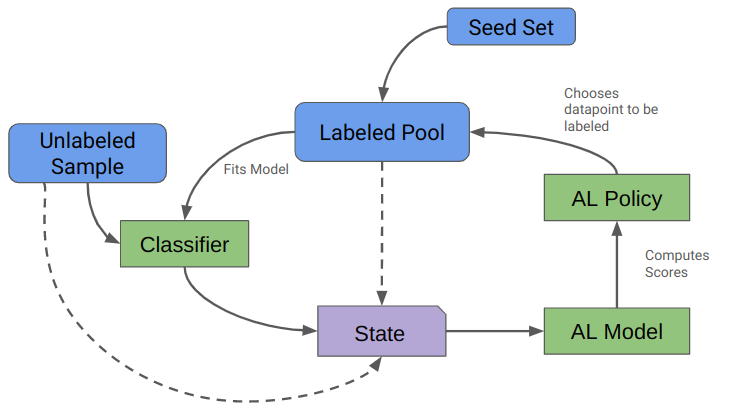
\includegraphics[width=\linewidth]{pics/al_cycle.png}
	\end{figure}
\end{frame}

%%%%%%%%%%%%%%%%%%%%%%%%%%%%%%%%%%%%%%%%%%%%%%%%%%%%%%%%%%%%%%%%%%%%%%%%%%%%%%%%%%%%%%%%%%%%%%%%%%

\begin{frame}[fragile]{Datasets}
	Each dataset should be preprocessed - The features are normalized, the target are one-hot encoded and \textbf{the seed set should be fixed}
	
	Datasets should be selected by their "potential"
	
	Each dataset needs an oracle curve that sets an upper bound performance
\end{frame}

%%%%%%%%%%%%%%%%%%%%%%%%%%%%%%%%%%%%%%%%%%%%%%%%%%%%%%%%%%%%%%%%%%%%%%%%%%%%%%%%%%%%%%%%%%%%%%%%%%

\begin{frame}[fragile]{Classifier}
	The classification model should be governed by the dataset 
	
	There is no need to have the same model for every dataset, as long as the model in question is suited well for the data 
	
	Simpler models with less dynamic behaviour are better - SOTA performance is not so important
	
	The model needs have tuned hyperparameters for each dataset (full dataset or subset?)
	
	The expectation is that good AL algorithms will also work well on SOTA models
	%Adam vs. SGD?
\end{frame}

%%%%%%%%%%%%%%%%%%%%%%%%%%%%%%%%%%%%%%%%%%%%%%%%%%%%%%%%%%%%%%%%%%%%%%%%%%%%%%%%%%%%%%%%%%%%%%%%%%

\begin{frame}[fragile]{Evaluation Metrics}
	Multiple options are available
	\begin{itemize}
		\item Accuracy* / F1-Score
		\item AUC
		\item Advantage over random sampling*
		\item Regret from the oracle curve
		\item Relative performance (0\% = random / 100\% = oracle)
	\end{itemize}
\end{frame}

%%%%%%%%%%%%%%%%%%%%%%%%%%%%%%%%%%%%%%%%%%%%%%%%%%%%%%%%%%%%%%%%%%%%%%%%%%%%%%%%%%%%%%%%%%%%%%%%%%

\begin{frame}[fragile]{Cross Validation}
	Splice: 
	random 0.874 +- 0.01
	margin 0.885 +- 0.015
	difference 0.011
	Changing the data vs. changing the model initialization
\end{frame}

%%%%%%%%%%%%%%%%%%%%%%%%%%%%%%%%%%%%%%%%%%%%%%%%%%%%%%%%%%%%%%%%%%%%%%%%%%%%%%%%%%%%%%%%%%%%%%%%%%

\begin{frame}[fragile]{Hyperparameters}
	Data HPs are fixed by the dataset (budget, seed set, ...)
	
	Classifier HPs are set with BO per dataset (architecture, learning rate, regularization, ...)
	
	Environment HPs are choosen with respect to the classifiers (training loop, ...)
	
	Each AL agent defines its own state space with the information from the environment
	
	This leaves very few "true" hyperparameters: 
	\begin{itemize}
		\item Unlabeled Sample Size
		\item \# of cross validation trials
	\end{itemize}
\end{frame}

%%%%%%%%%%%%%%%%%%%%%%%%%%%%%%%%%%%%%%%%%%%%%%%%%%%%%%%%%%%%%%%%%%%%%%%%%%%%%%%%%%%%%%%%%%%%%%%%%%

\begin{frame}[fragile]{Single Domain vs. Transfer}
	pass
\end{frame}


\end{document}
